% Importé depuis Chapitre.docx (partie 1)
\PFEChapterOpening{Etude préalable}
\pagestyle{fancy}
\markboth{Chapitre 1 : Etude préalable}{}
% Force l'en-tête du chapitre 1 sur toutes ses pages.
\fancyhead[L]{\textcolor{ISGGray}{Chapitre 1 : Etude préalable}}
\renewcommand{\headrulewidth}{0.6pt}
\renewcommand{\headrule}{%
  \hbox to\headwidth{%
    \color{ISGGray}\leaders\hrule height \headrulewidth\hfill
  }%
}

\section{Introduction}
\begingroup
\noindent
Ce premier chapitre est consacré à l’étude préalable du projet. Il présente l’organisme d’accueil ainsi que le cadre général du projet, en mettant en évidence la problématique, la mission et les objectifs de la plateforme. Il aborde ensuite l’étude de l’existant et la solution proposée. Enfin, il propose une présentation des méthodologies de gestion de projet, notamment les méthodes agiles, avant de préciser et de justifier le choix de la méthodologie adoptée.
\section{Présentation de l’organisme d’accueil}
Notre stage a été effectué au sein de COFICAB, filiale du Groupe Elloumi, acteur majeur de la fabrication de câbles pour l’industrie automobile.
\subsection{Présentation de groupe ELLOUMI}%
Le Groupe Elloumi \cite{elloumi-website}, fondé en 1946 par M.Taoufik Elloumi, s'impose aujourd'hui comme le plus grand groupe industriel et exportateur tunisien, avec environ 30 filiales à travers le monde. Le groupe intervient dans de nombreux secteurs câbles et composants automobiles, électroménager notamment à travers sa filiale COFICAB.

La figure 1.1 présente la structure du groupe ELLOUMI.
\vspace{-0.35\baselineskip}% léger resserrement avant la figure
\endgroup
\begin{figure}[H]
  \centering
  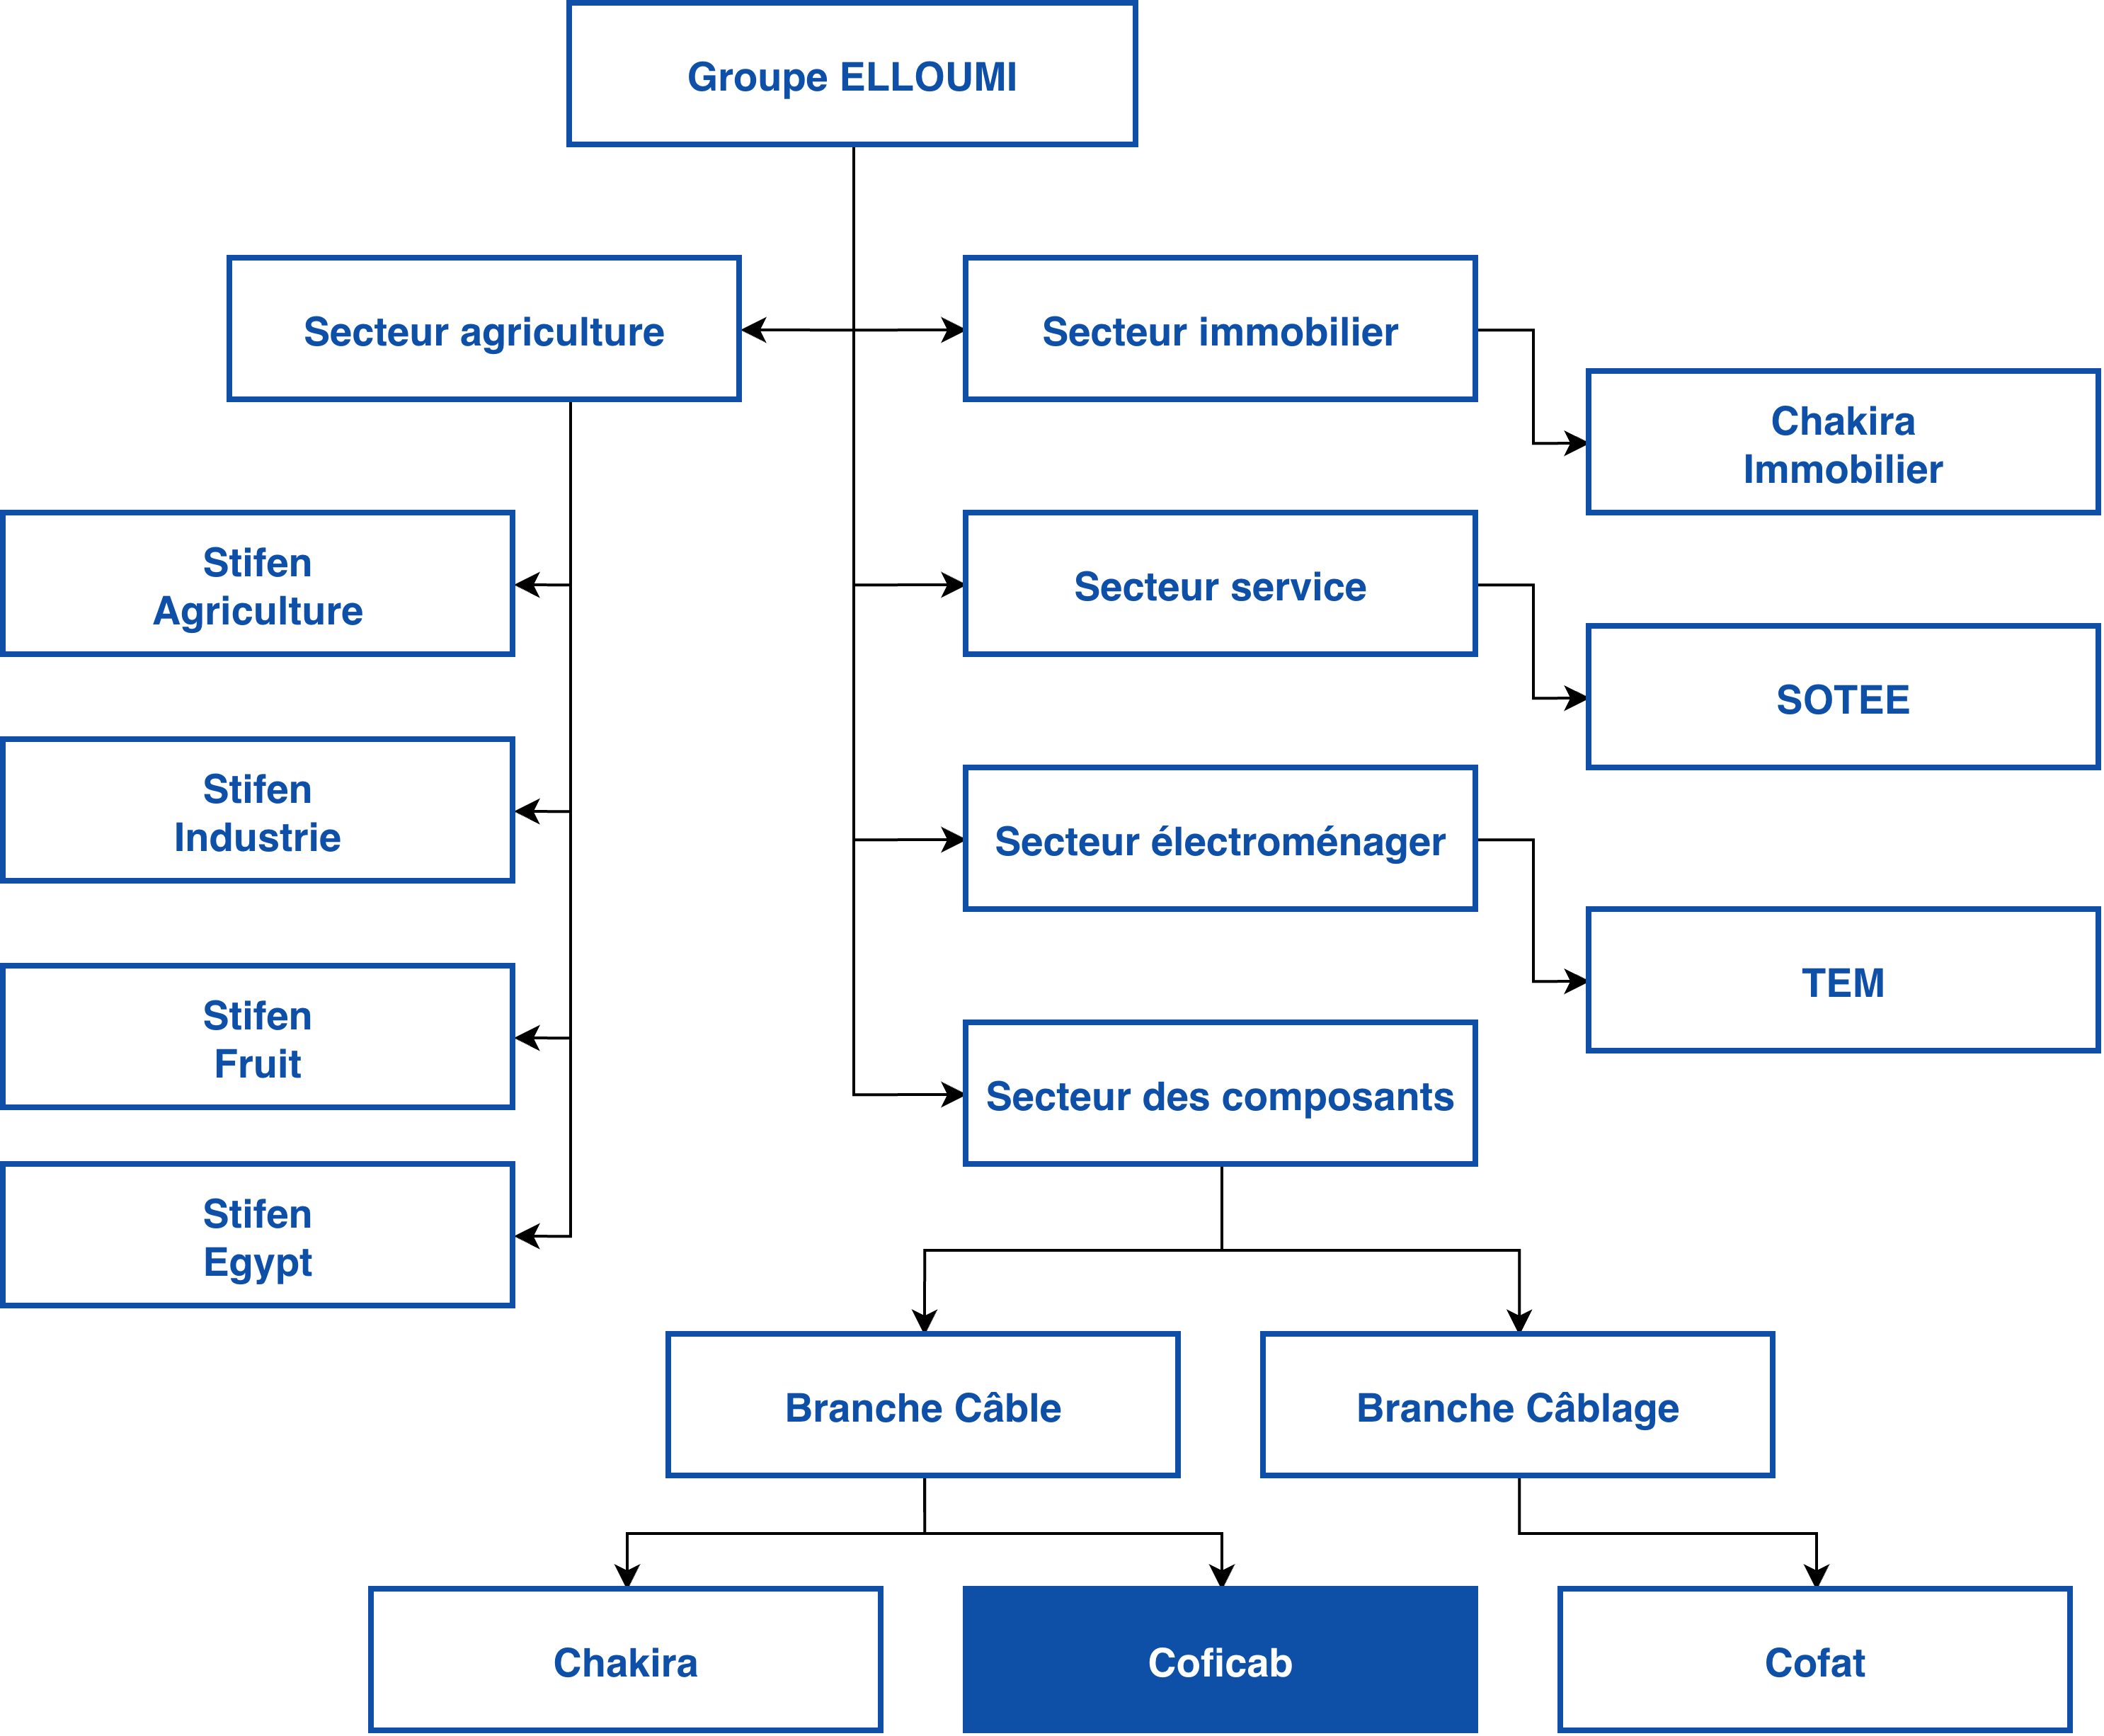
\includegraphics[width=0.78\linewidth]{figures/chapitre-01/groupe_elloumi.png}
  \caption{Organigramme du groupe Elloumi.}
  \label{fig:Organigramme_groupe_Elloumi}
\end{figure}

\subsection{Présentation de l’entreprise COFICAB}
COFICAB \cite{coficab-website} est une entreprise industrielle internationale fondée en 1992 et  spécialisée dans la conception, la fabrication et la commercialisation de câbles et fils électriques pour l’industrie automobile. Elle détient environ 23\% de part de marché mondiale et accompagne les évolutions technologiques du secteur, notamment en mobilité électrique, sécurité et performance. Grâce à une implantation internationale couvrant quatre continents et seize pays, COFICAB opère à travers un réseau structuré de sites industriels, de centres de recherche et d’unités commerciales, employant environ 9 000 collaborateurs.

La figure 1.2 présente le logo de la société COFICAB.
\vspace{0.5cm}
\begin{figure}[H]
  \centering
  
\includegraphics[width=0.4\linewidth]{figures/chapitre-01/coficab-logo.png}
  \caption{Logo de COFICAB.}
  \label{fig:Logo_Coficab}
\end{figure}
Pour mieux comprendre la stratégie de COFICAB, il est essentiel d’analyser l’implantation de ses unités de production, ce qui permet de mettre en évidence sa stratégie territoriale et son positionnement sur les marchés \cite{global-footprint-coficab}.

La figure 1.3 présente la répartition géographique des sites de COFICAB.


\begin{figure}[H]
  \centering
  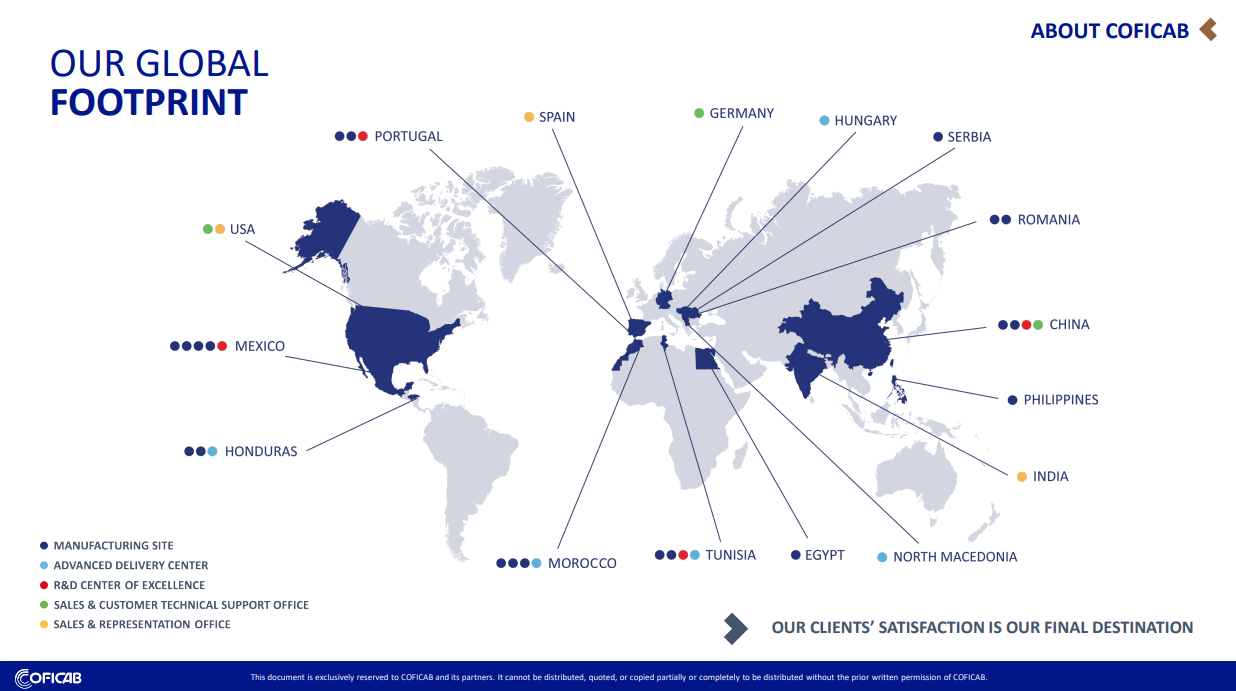
\includegraphics[width=1\linewidth]{figures/chapitre-01/global_footprint_coficab.png}
  \caption{Implantations géographiques de COFICAB.}
  \label{fig:doc-ch1-3}
\end{figure}

\subsection{Outils de gestion utilisés au sein de la société}
Afin d’assurer une gestion efficace et structurée de ses activités, COFICAB s’appuie sur des outils de gestion modernes et intégrés, permettant d’optimiser les processus internes, de faciliter la prise de décision et d’améliorer la performance globale de l’entreprise.
Les principaux outils utilisés sont :

\begin{itemize}[label=\textbullet]
  \item \textbf{Odoo \cite{odoo-docs}} : pour la gestion intégrée des processus de production, logistique, ressources humaines et finance.
  \item \textbf{Power BI \cite{powerbi-docs}} : pour le pilotage de la performance, la création de tableaux de bord et le suivi des KPI\footnote{KPI : \emph{Key Performance Indicator} (indicateur clé de performance). Il s’agit de mesures quantitatives permettant d’évaluer l’atteinte des objectifs et de piloter la performance organisationnelle ou opérationnelle.}.
  \item \textbf{MES\footnote{MES : \emph{Manufacturing Execution System}. Il s’agit d’un système d’exécution de la production permettant de suivre et piloter les opérations de fabrication en temps réel (traçabilité, contrôle, collecte des données de production, indicateurs).} \cite{mes-docs}} : pour le suivi en temps réel des opérations de production, la traçabilité des produits et le contrôle des processus industriels.
  \item \textbf{Trello \cite{trello-docs}} : pour faciliter la communication interne, la gestion documentaire et le travail en équipe.
\end{itemize}
L’utilisation combinée de ces outils contribue à l’amélioration continue des processus, à l’optimisation des performances et au maintien de la compétitivité internationale de COFICAB.

\section{Cadre général du projet}

\subsection{Problématique}

Face aux enjeux croissants liés à la Responsabilité Sociale des Entreprises (RSE) et à la nécessité d’un pilotage performant des actions environnementales, sociales et de gouvernance, les grandes organisations industrielles doivent aujourd’hui disposer de systèmes d’information fiables, centralisés et orientés décision. La multiplication des sites, la diversité des initiatives RSE et l’exigence de reporting structuré rendent les méthodes traditionnelles basées sur des fichiers Excel et des échanges par emails insuffisants pour assurer un suivi efficace et cohérent.

Dans ce contexte, la société COFICAB a exprimé le besoin de mettre en place une solution permettant de planifier, suivre, consolider et analyser les activités RSE à l’échelle de l’ensemble de ses sites.

\subsection{Définition de la mission}

Le présent projet consiste à concevoir et développer une plateforme RSE centralisée, destinée à améliorer la gouvernance, la visibilité et la prise de décision au niveau corporate. La mission principale de ce projet est de :


\begin{itemize}[label=\textbullet, itemsep=0.15ex, parsep=0pt, topsep=0pt, partopsep=0pt]
  \item Concevoir une plateforme web permettant la planification annuelle des activités RSE par site avec un processus de validation structuré.
  \item Assurer le suivi en temps réel des activités réalisées, incluant les activités hors plan.
  \item Centraliser les données RSE afin de fournir une vue consolidée au niveau corporate.
  \item Mettre en place des tableaux de bord Power BI et des indicateurs clés de performance (KPI) Power BI afin d’analyser le taux de réalisation des plans, les budgets des activités, la participation... 
  \item Faciliter l’analyse historique et la gestion des changements à travers un mécanisme de demandes de modification pour les périodes clôturées
\end{itemize}

Cette plateforme vise ainsi à renforcer la performance RSE de COFICAB, à fiabiliser le reporting et à soutenir la prise de décision stratégique grâce à une exploitation optimale des données.

\subsection{Objectifs à atteindre}

Les principaux objectifs que nous visons à atteindre à travers notre application sont :

\begin{enumerate}
  \item \textbf{Centraliser et structurer la gestion des activités des sites dans une plateforme unique}.
  \item \textbf{Fiabiliser le suivi des plans et des activités sur l’ensemble du cycle de vie} avec un workflow de validation, des statuts maîtrisés et une historisation des opérations.
  \item \textbf{Renforcer le contrôle d’accès et la sécurité des données sensibles} par une authentification sécurisée, une gestion des rôles et une restriction d’accès par site.
  \item \textbf{Améliorer la gestion des demandes de modification et la traçabilité des actions} sur les périodes clôturées et les données déjà validées.
  \item \textbf{Assurer une traçabilité complète des opérations via un journal d’audit (log)} pour suivre les créations, modifications, validations, rejets et suppressions.
  \item \textbf{Intégrer un chatbot d’assistance intelligent} pour guider les utilisateurs, répondre aux questions fréquentes et faciliter l’accès rapide aux informations clés de la plateforme.
  \item \textbf{Optimiser le reporting et l’analyse des performances CSR} par la comparaison planifié/réalisé, le calcul automatique des KPI et des tableaux de bord dynamiques.
\end{enumerate}

\section{Étude de l’existant}

\subsection{Analyse de l’existant}

\subsubsection{Description de la gestion des activités RSE au niveau de COFICAB}

La gestion des activités RSE au sein de COFICAB repose sur une organisation fortement décentralisée et peu structurée. Chaque site industriel gérait de manière autonome ses activités RSE, depuis la phase de planification jusqu’au suivi de leur réalisation, sans cadre unifié ni outil centralisé permettant d’harmoniser les pratiques.

Concrètement, les responsables RSE au niveau des différents sites utilisaient principalement des outils bureautiques classiques, notamment des fichiers Excel pour la planification annuelle (\textit{CSR Plan}), la saisie des données réelles des activités (\textit{CSR Report}) et la consolidation globale (\textit{CSR consolidé}) permettant le calcul des KPIs.

\begin{itemize}[label=\textbullet, itemsep=0.15ex, parsep=0pt, topsep=0pt, partopsep=0pt]
  \item Le CSR Plan représente le plan annuel élaboré par le responsable RSE de chaque site, puis soumis à un processus de validation selon le mode de validation défini. Ce plan regroupe les informations essentielles nécessaires au suivi et à la gestion des activités RSE, notamment l’identifiant du plan, le site concerné, l’année de référence, le mode de validation, le budget alloué ainsi que l’effectif total du site.
  Les activités planifiées associées à ce plan sont décrites à travers plusieurs informations, notamment l’identifiant de l’activité, la catégorie, le partenaire externe éventuel, l’intitulé, l’organisation, le type de contrat, la description, la nature de la collaboration, la périodicité, le budget prévu, l’objectif d’impact, l’unité d’impact, la durée de l’impact, le nombre d’employés impliqués, l’année de démarrage, le numéro d’édition et l’organisateur.
  
  La figure~\ref{fig:doc-ch1-csr-plan-workflow} présente le tableau du plan annuel CSR utilisé pour la planification des activités.
  \begin{figure}[H]
  \centering
  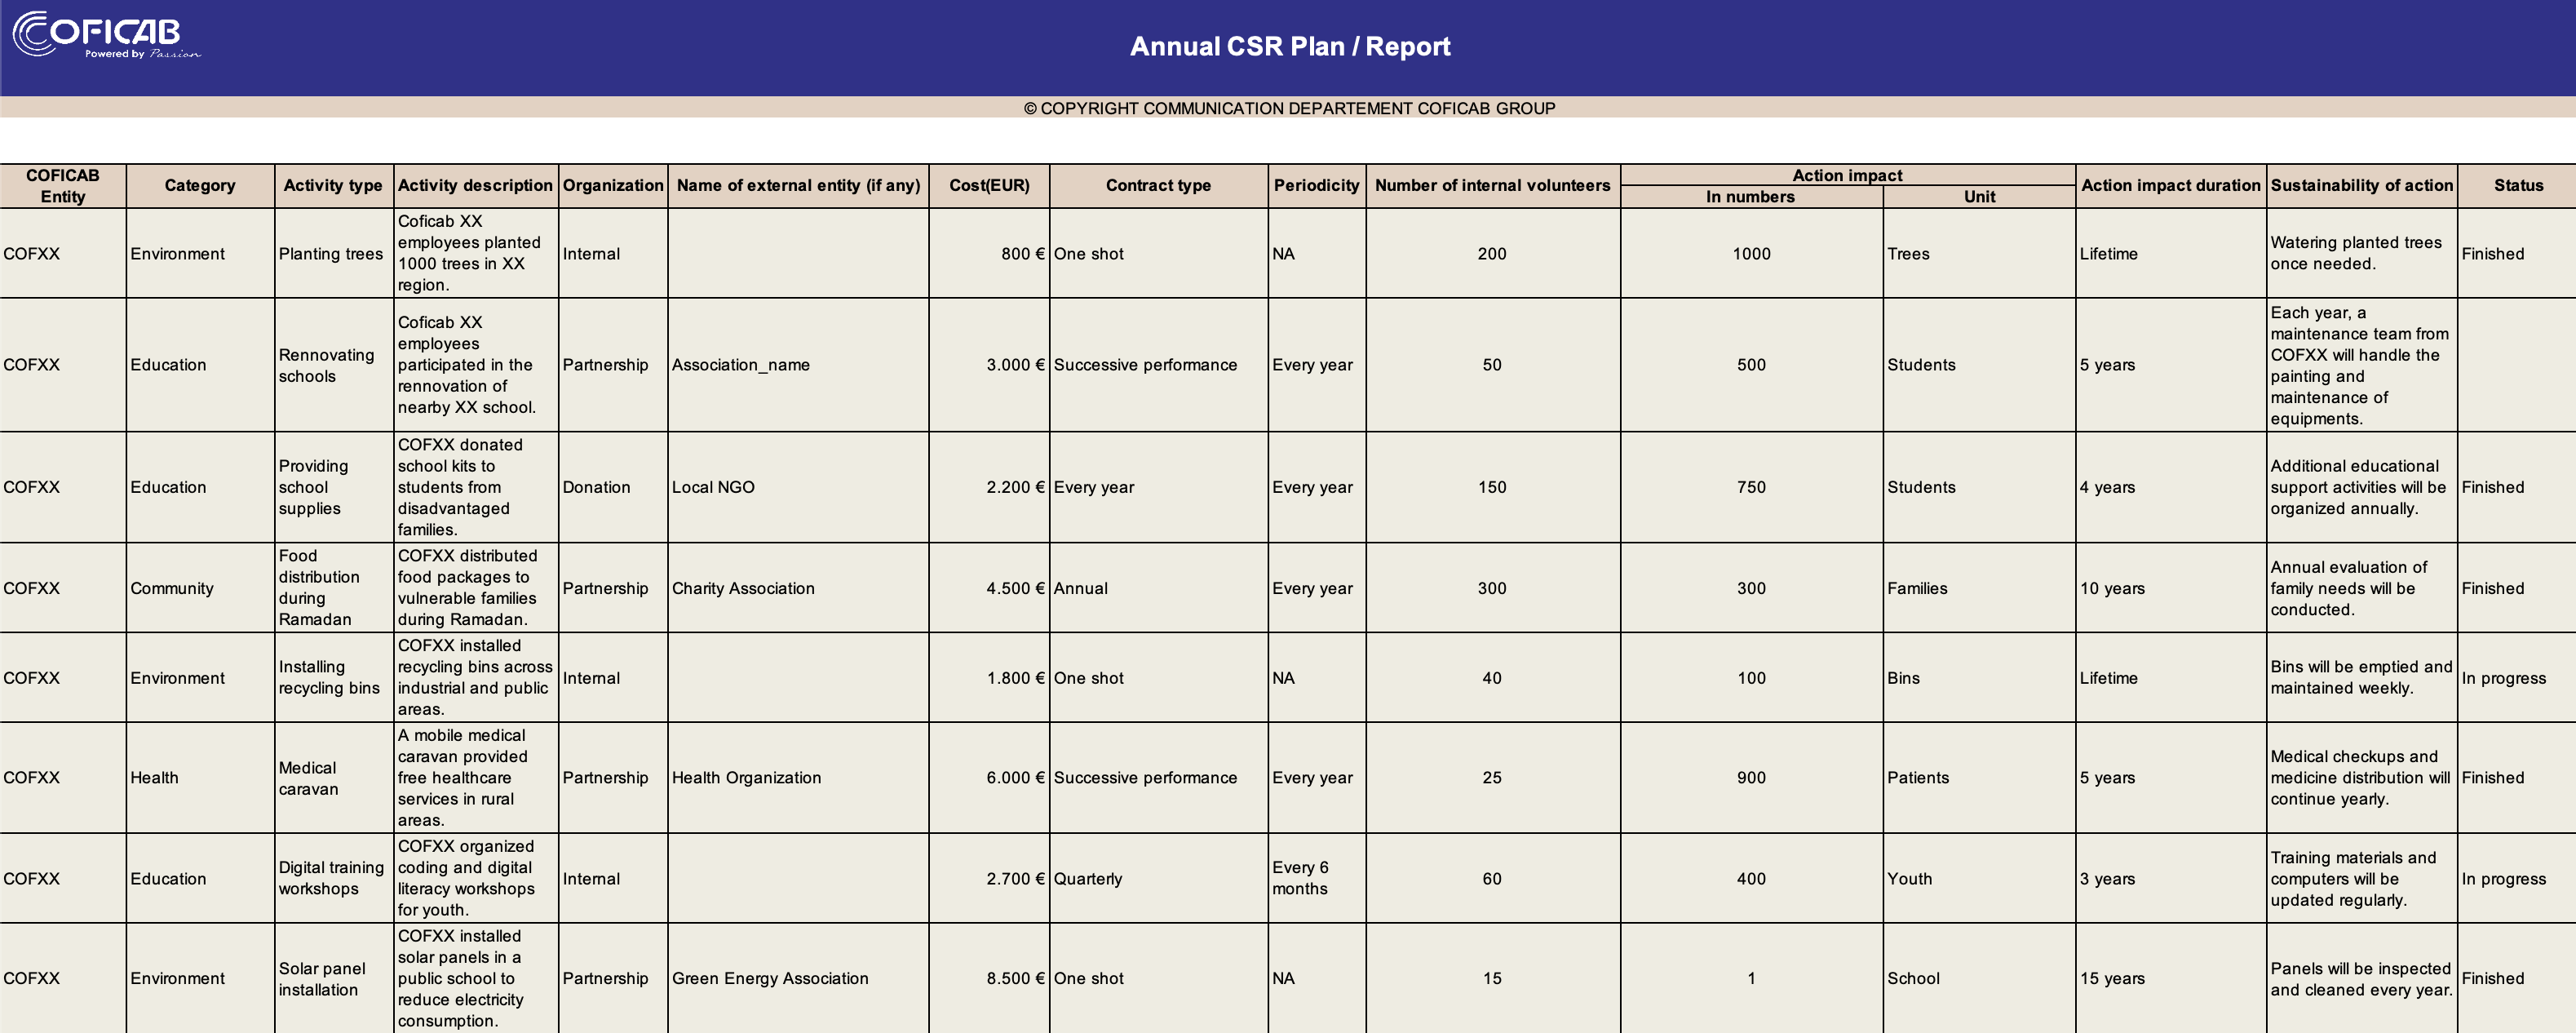
\includegraphics[width=1\linewidth]{figures/chapitre-01/annual-csr-plan.png}
  \caption{Tableau du plan annuel CSR utilisé pour la planification des activités.}
  \label{fig:doc-ch1-csr-plan-workflow}
\end{figure}
\newpage
 \item Le CSR Report correspond aux données réelles des activités réalisées. Il regroupe les informations essentielles liées à chaque activité, telles que l’activité, le nombre de participants, le nombre de participants internes, les indicateurs d’impact, le nombre d’incidents, le département du contact, le budget réellement dépensé, l’impact réalisé, l’unité d’impact, la date de réalisation ainsi que les informations de contact.
 
 La figure~\ref{fig:doc-ch1-csr-report-workflow} présente la formulaire du rapport des activités de contribution sociale.
 \begin{figure}[H]
  \centering
  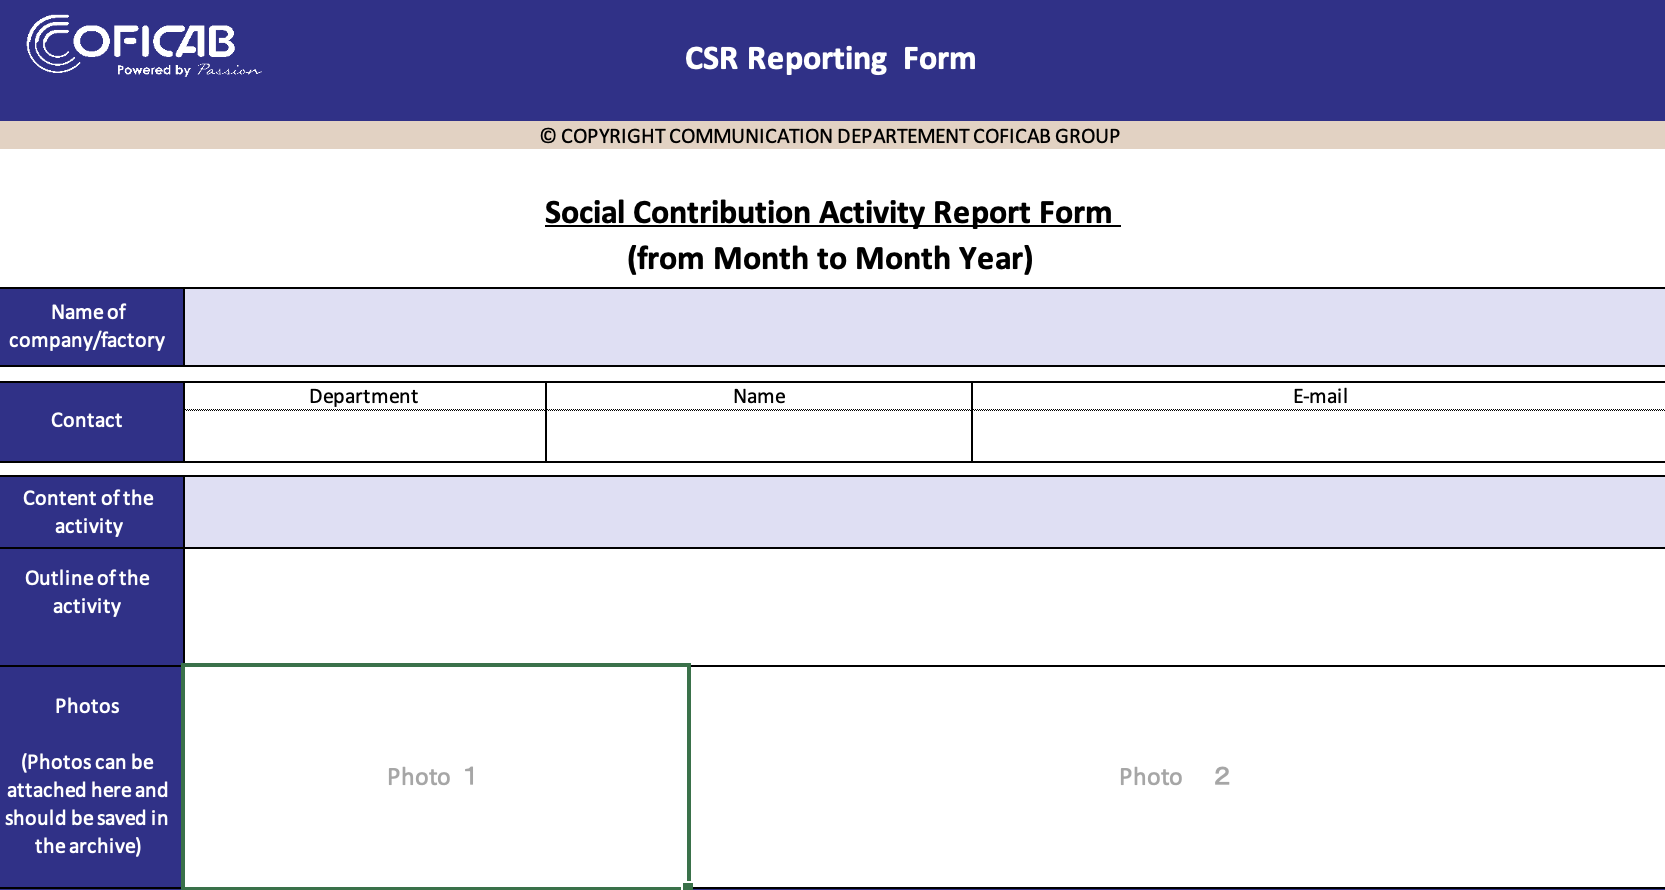
\includegraphics[width=0.9\linewidth]{figures/chapitre-01/csr-report.png}
  \caption{Formulaire du rapport des activités de contribution sociale}
  \label{fig:doc-ch1-csr-report-workflow}
\end{figure}

\item Le CSR Consolidé offre une vue synthétique de l’ensemble des activités RSE réalisées. Il permet de comparer les budgets prévus et réels, d’évaluer les impacts générés et de suivre l’implication des parties prenantes internes et externes. Il constitue un outil de pilotage global facilitant l’analyse et le suivi des performances RSE à l’échelle de l’organisation, en intégrant le calcul des principaux KPI.

La figure~\ref{fig:doc-ch1-csr-kpi-realise} présente le tableau consolidé des activités CSR réalisées.
\begin{figure}[H]
  \centering
  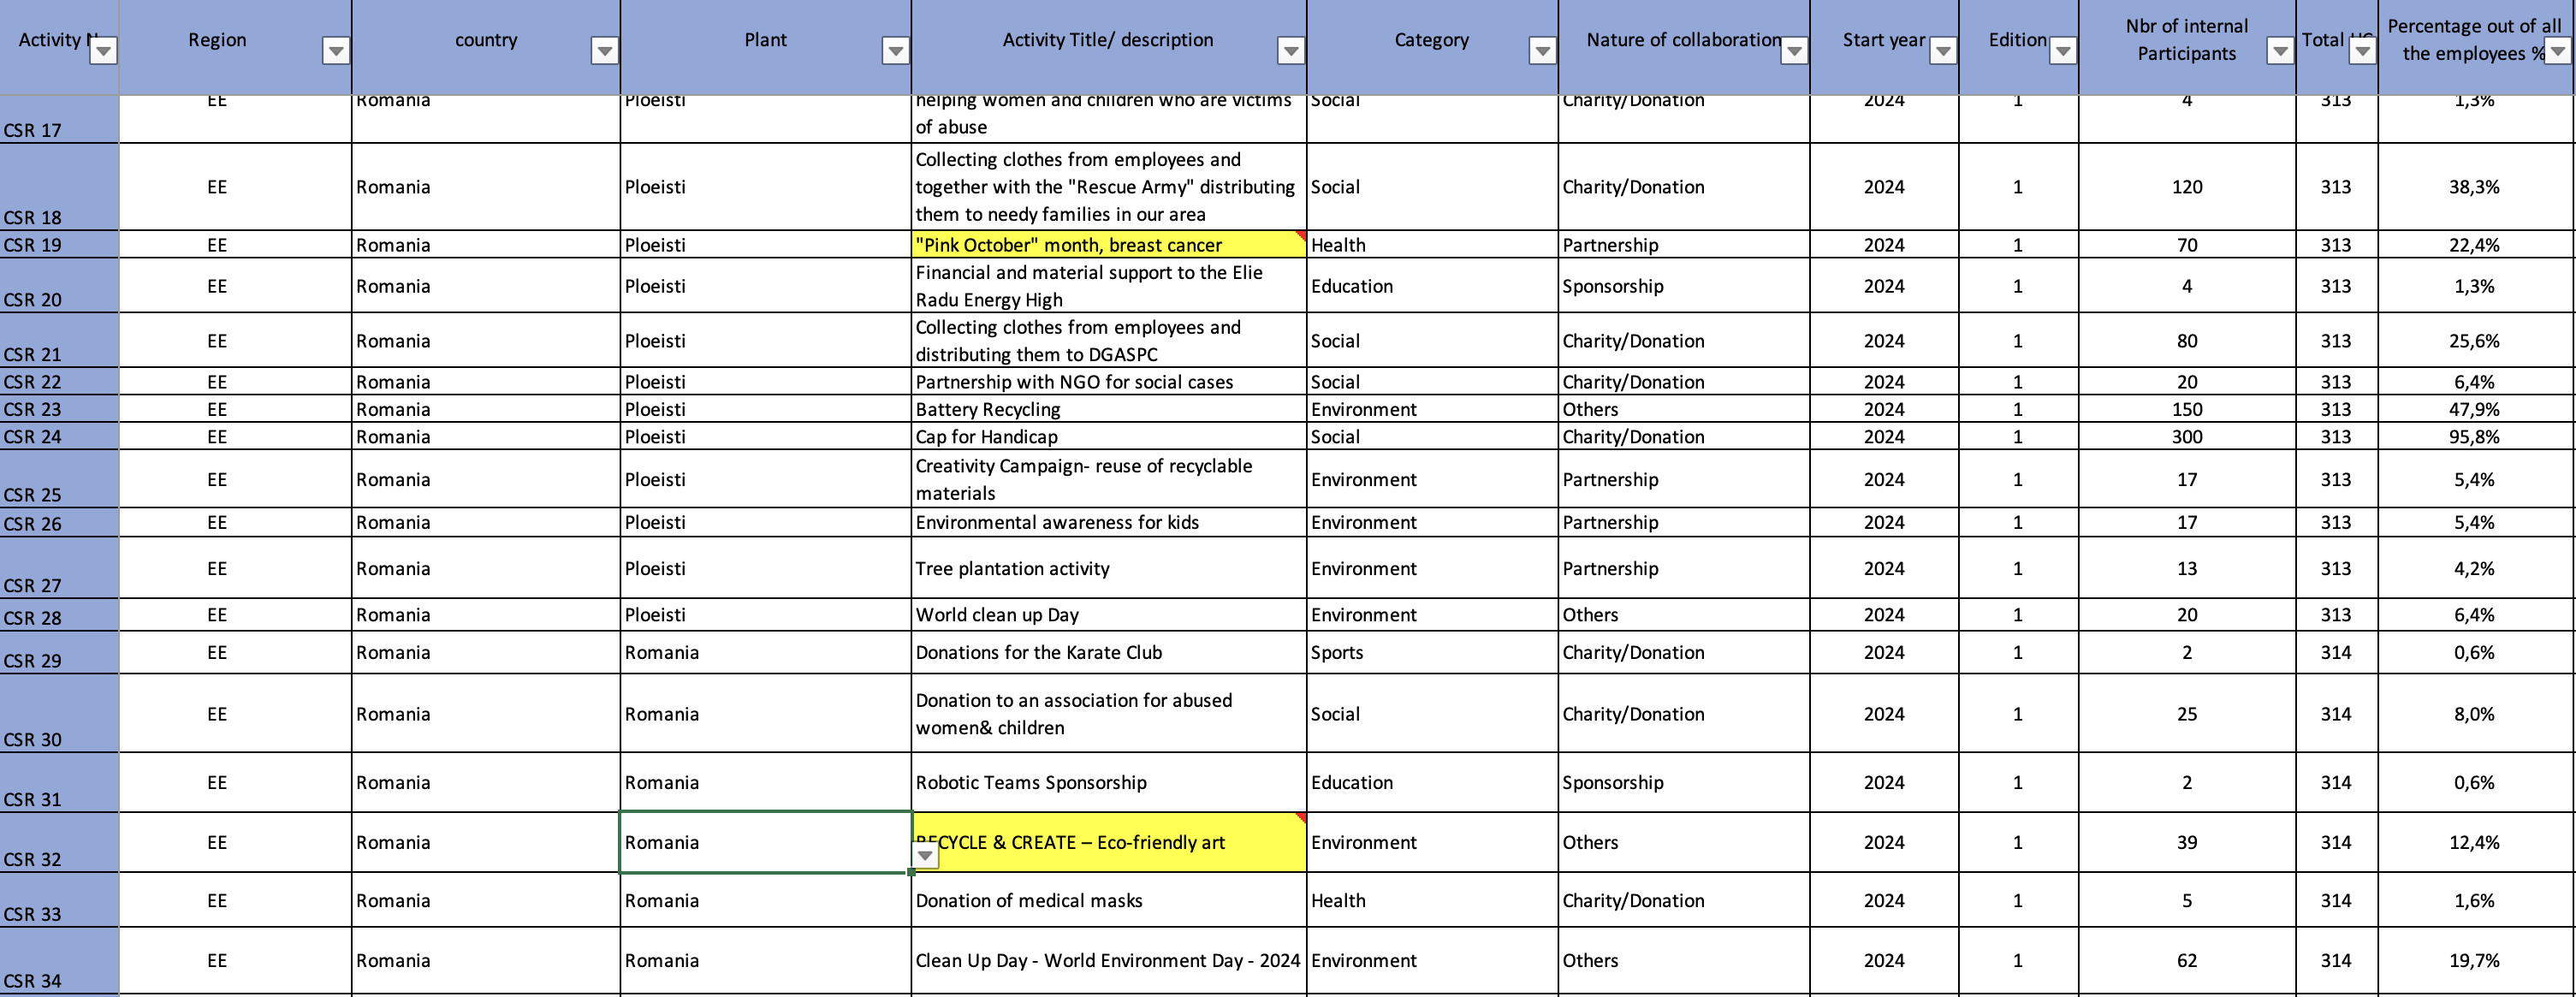
\includegraphics[width=1\linewidth]{figures/chapitre-01/kpi-tout-activitties.png}
  \caption{Tableau consolidé des activités CSR réalisées}
  \label{fig:doc-ch1-csr-kpi-realise}
\end{figure}
\end{itemize}

La figure~\ref{fig:doc-ch1-csr-kpi-workflow} présente un exemple des KPIs calculés à partir du tableau consolidé.
\begin{figure}[H]
  \centering
  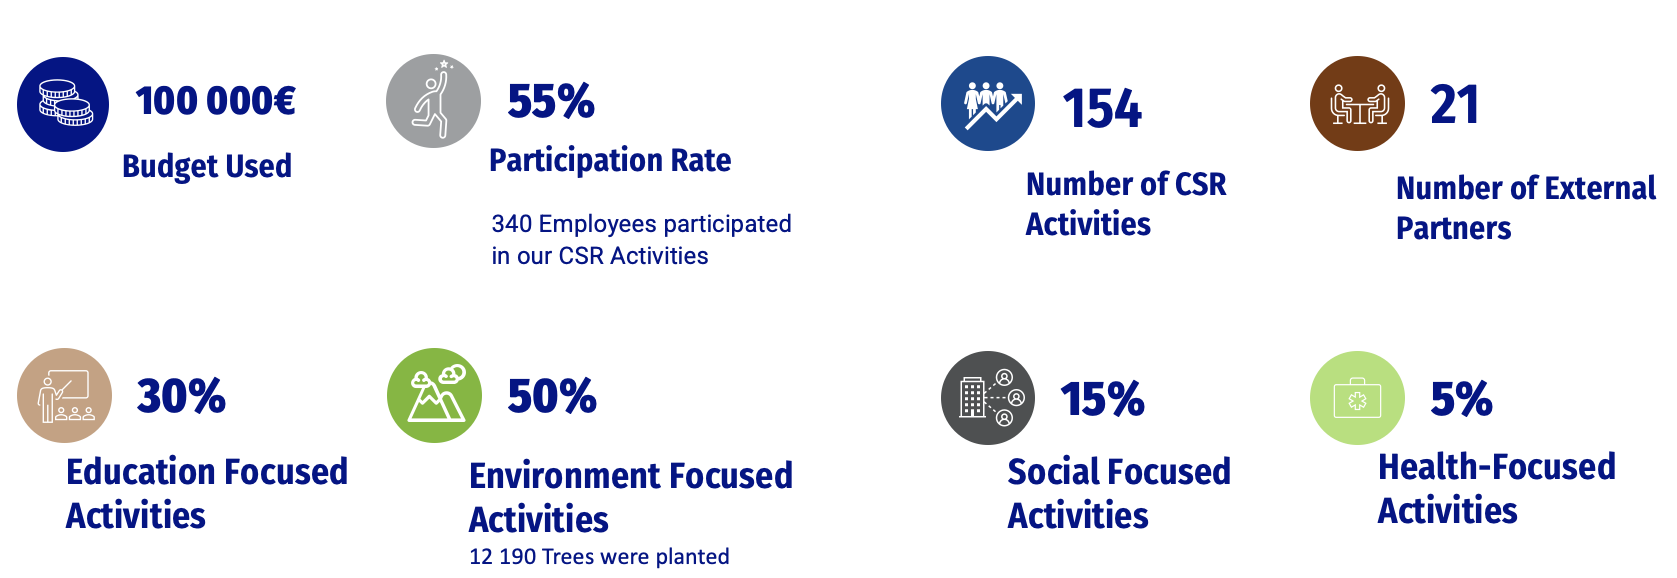
\includegraphics[width=0.9\linewidth]{figures/chapitre-01/exemple-kpi.png}
  \caption{Exemple des KPIs calculés à partir du tableau consolidé.}
  \label{fig:doc-ch1-csr-kpi-workflow}
\end{figure}

Les échanges d’informations se faisaient principalement par email, tandis que chaque site utilisait ses propres formats de fichiers, indicateurs et méthodes de calcul. Les données étaient ensuite regroupées et harmonisées afin de permettre le suivi global des activités RSE et la comparaison entre les différents sites.

Le processus de gestion des activités RSE ne reposait pas sur un workflow de validation formalisé, tandis que le suivi des activités et le reporting étaient réalisés manuellement à partir de plusieurs sources.

La figure~\ref{fig:doc-ch1-workflow-processus-actuel} présente la processus actuel de gestion des activités RSE chez COFICAB.
\begin{figure}[H]
  \centering
  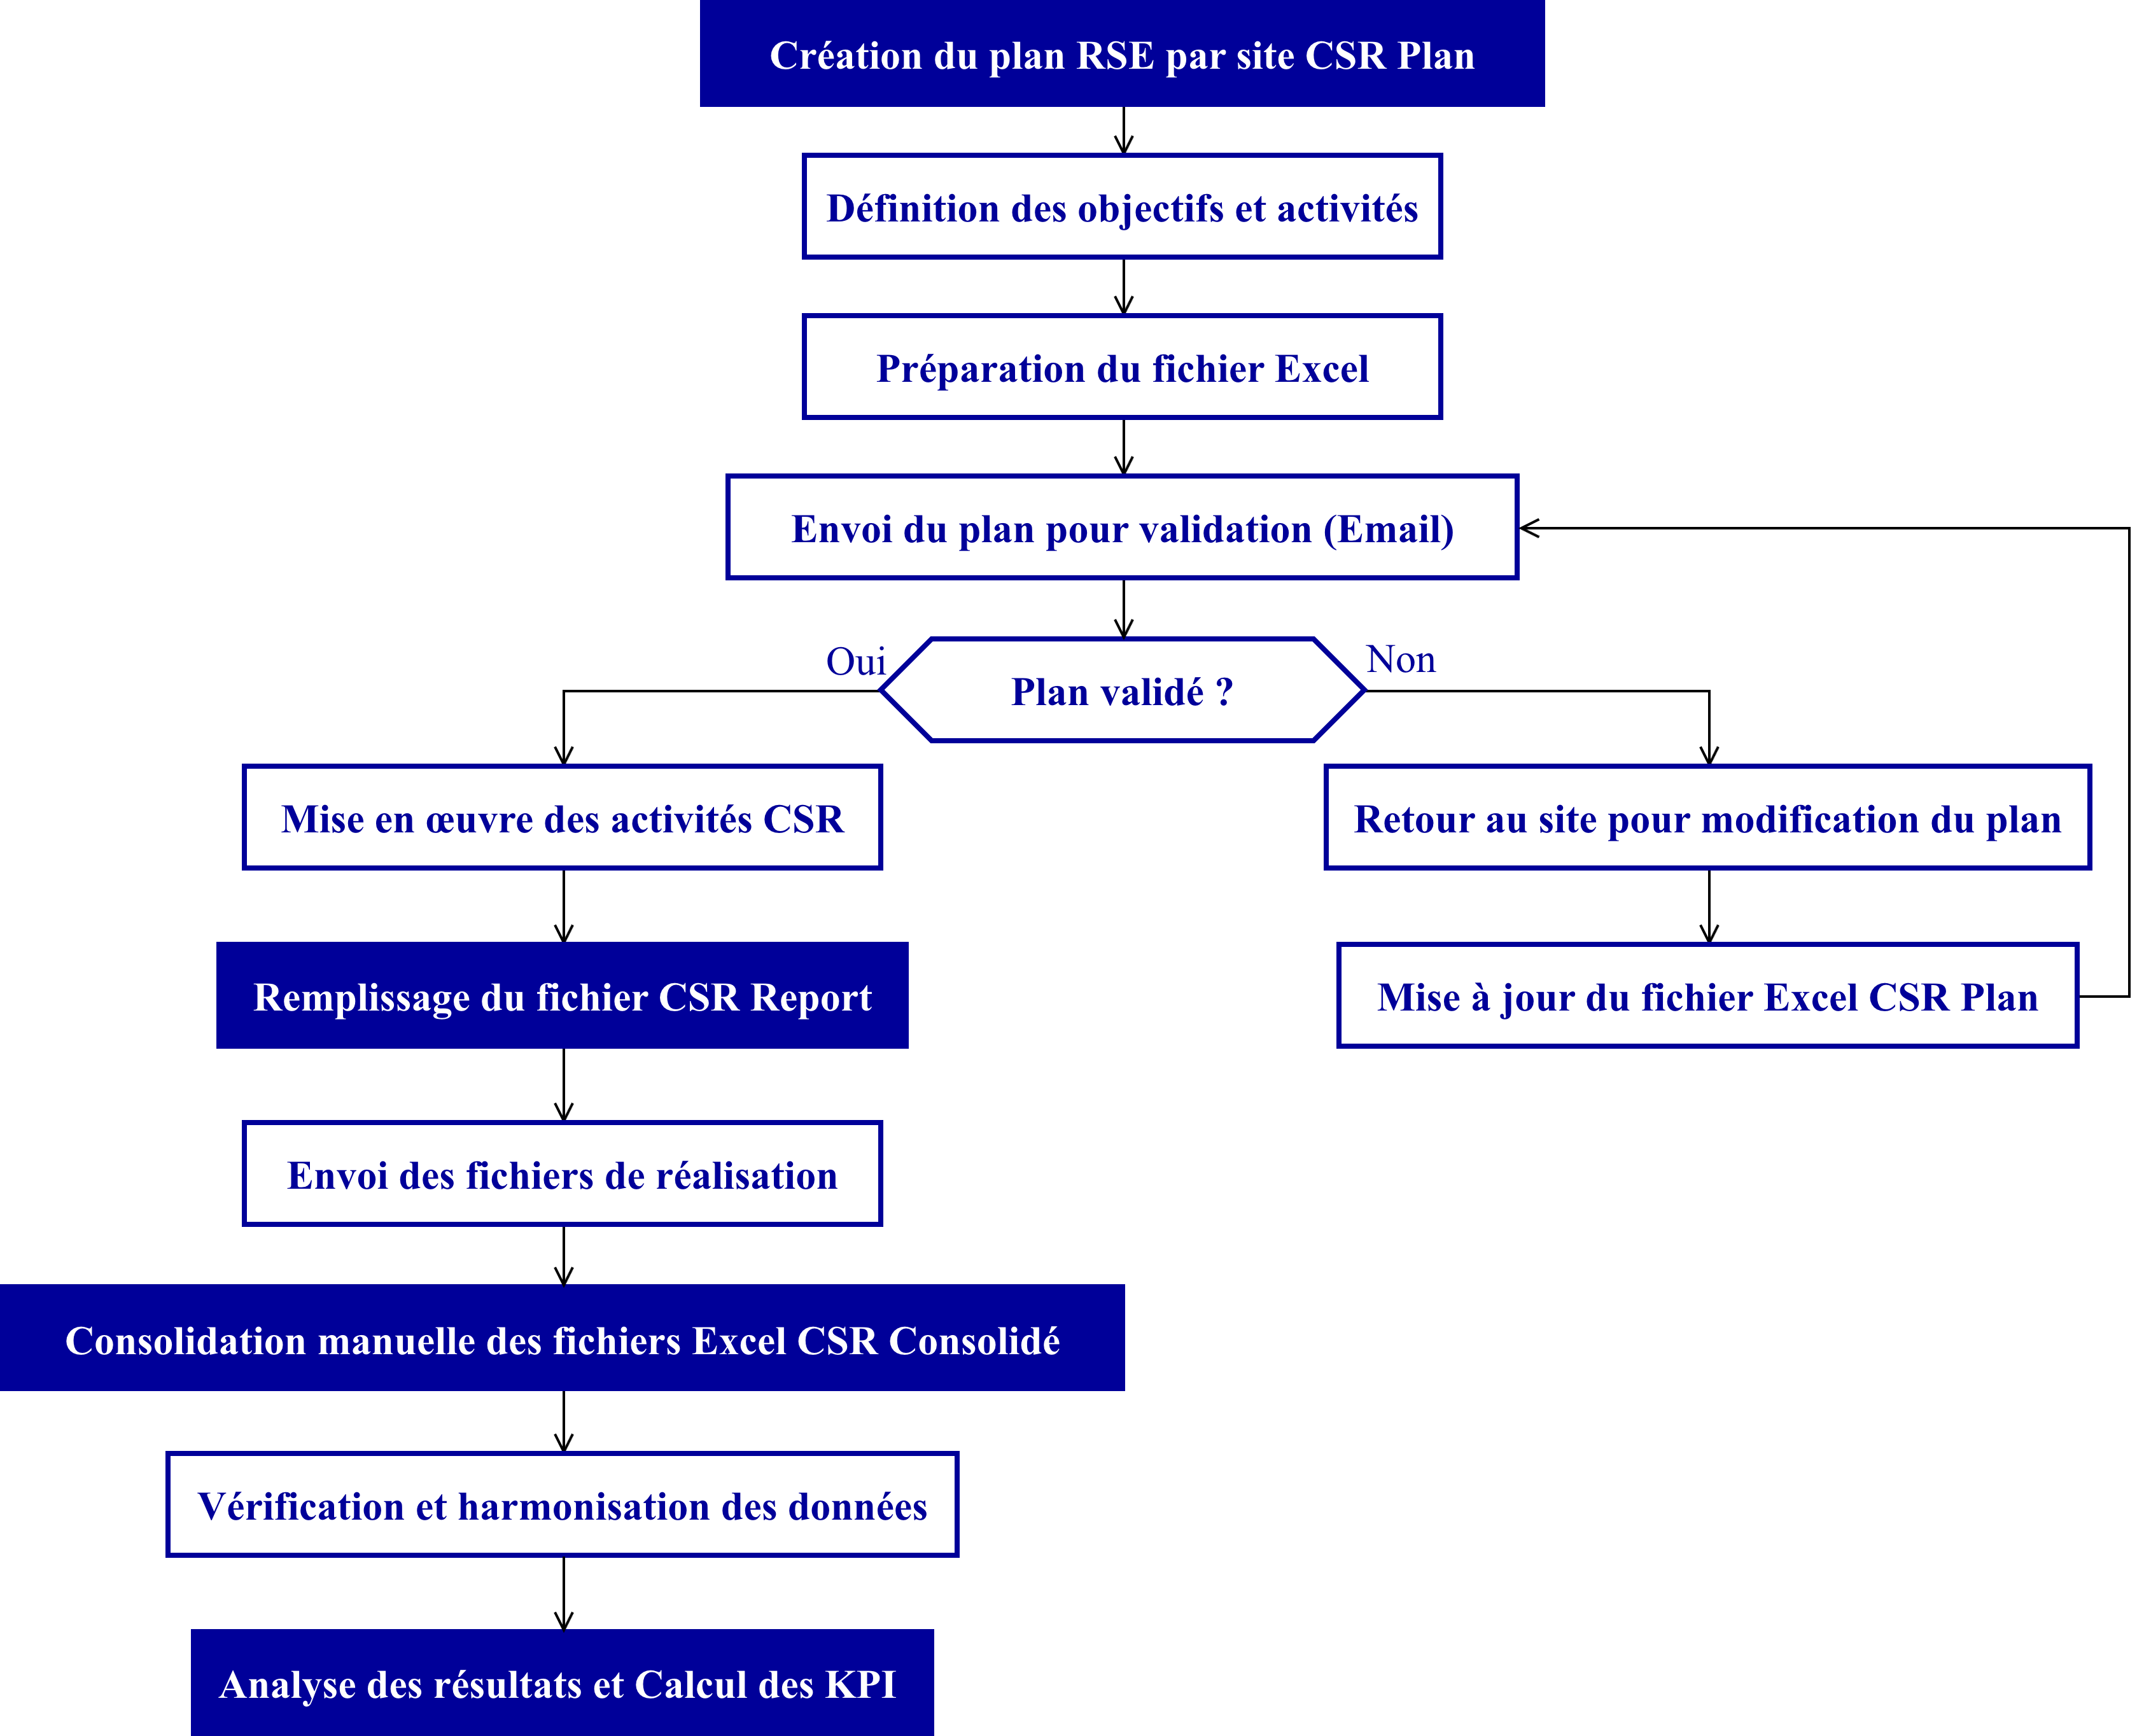
\includegraphics[width=0.85\linewidth]{figures/chapitre-01/workflow_prosessus_actuelle.png}
  \caption{Processus actuel de gestion des activités RSE chez COFICAB.}
  \label{fig:doc-ch1-workflow-processus-actuel}
\end{figure}

\newpage
\subsubsection{Description d’applications d’analyse d’activité RSE similaires}
\begin{itemize}[label=\textbullet]
  \item \textbf{Generous Connect :} \url{www.generousconnect.com}
\end{itemize}


Generous Connect \cite{Generous-Connect} est une plateforme numérique dédiée à la gestion et au suivi des initiatives de responsabilité sociétale des entreprises. Elle permet aux organisations de planifier, coordonner et analyser les activités sociales et environnementales réalisées au sein de leurs sites.

La figure~\ref{fig:doc-ch1-4} présente un aperçu de l’interface de statistiques de Generous Connect.

\begin{figure}[H]
  \centering
  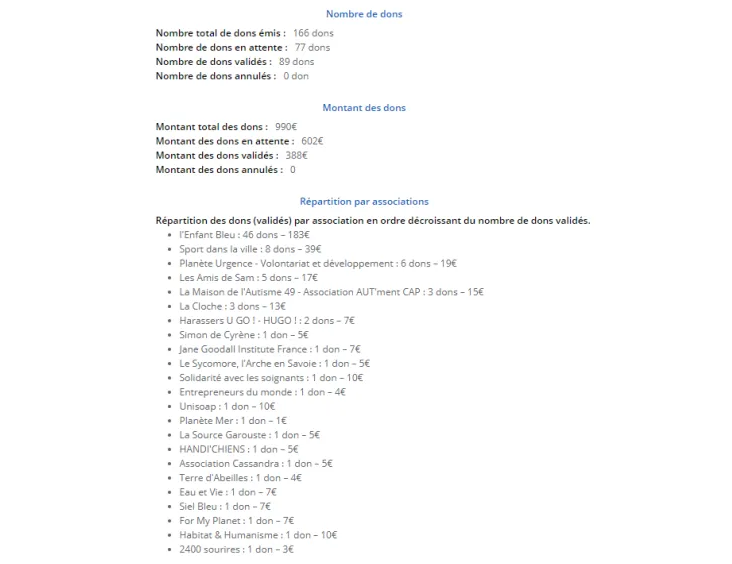
\includegraphics[width=1.1\linewidth]{figures/chapitre-01/generous-connect-statistiques.png}
  \caption{Aperçu de l’interface de statistiques de Generous Connect.}
  \label{fig:doc-ch1-4}
\end{figure}
L’application centralise les informations relatives aux projets RSE, telles que les actions menées, les ressources mobilisées et les indicateurs de performance. Grâce à des outils d’analyse et de reporting, les responsables peuvent suivre l’avancement des initiatives, évaluer leur impact et améliorer la gestion des programmes RSE à travers des tableaux de bord analytiques facilitant la prise de décision.

\newpage
\begin{itemize}[label=\textbullet]
  \item \textbf{Optimy : Solution d’efficacité en gestion de programmes :} \url{www.optimy.com}
\end{itemize}
Optimy \cite{Optimy} est une plateforme spécialisée dans la gestion et le suivi des programmes d’impact, notamment les initiatives de responsabilité sociétale des entreprises. Elle permet aux entreprises de planifier, organiser et gérer efficacement leurs projets sociaux, environnementaux ou de sponsoring.

La solution centralise les informations liées aux programmes, facilite le suivi des activités et permet de mesurer leur performance à l’aide d’indicateurs et de rapports analytiques. Grâce à ses outils de gestion et de reporting, Optimy aide les responsables à évaluer l’impact des initiatives et à améliorer la prise de décision dans la gestion des programmes RSE.

La figure~\ref{fig:doc-ch1-5} présente un aperçu du tableau de bord de la plateforme Optimy.

\begin{figure}[H]
  \centering
  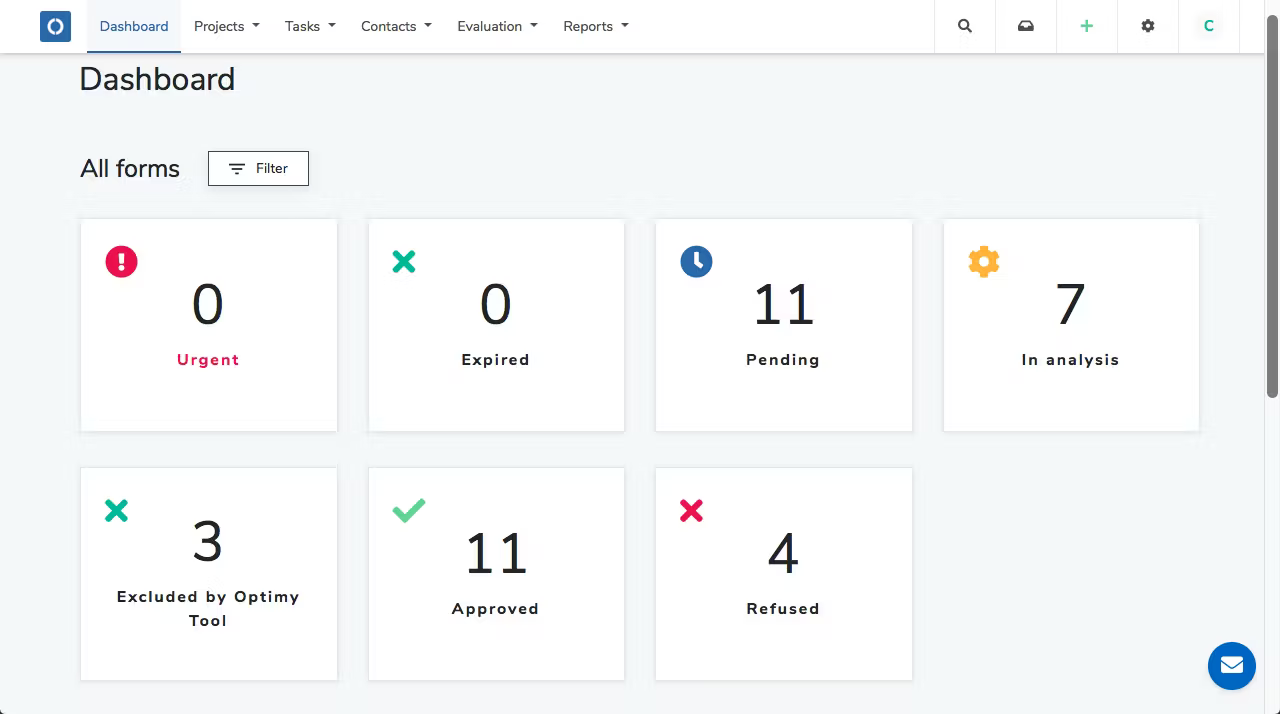
\includegraphics[width=1.1\linewidth]{figures/chapitre-01/optimy-dashboard.png}
  \caption{Aperçu du tableau de bord de la plateforme Optimy.}
  \label{fig:doc-ch1-5}
\end{figure}
\newpage
\subsection{Critique de l’existant}

\subsubsection{Critique des activités RSE au niveau de COFICAB}

L’analyse du système actuel de gestion des activités RSE au sein de COFICAB révèle plusieurs limites. 
\begin{itemize}[label=\textbullet, itemsep=0.15ex, parsep=0pt, topsep=0pt, partopsep=0pt]
  \item L’utilisation de fichiers Excel et de documents dispersés entraîne une gestion décentralisée et une hétérogénéité des données entre les différents sites. Cette situation rend difficile la consolidation des informations et limite la visibilité globale au niveau corporate.
  \item Le processus de validation des plans reste peu structuré (étapes, statuts, responsabilités), ce qui complique le suivi des approbations, allonge les délais de traitement et réduit la traçabilité des décisions.
  \item La comparaison entre les données planifiées et les données réelles n’est pas réalisée de manière systématique ni fiable, ce qui limite l’identification rapide des écarts de budget, d’impact et d’avancement des activités.
  \item Le reporting repose sur un traitement manuel des données, ce qui est chronophage et augmente le risque d’erreurs.
  \item L’absence d’un système centralisé et d’outils d’analyse adaptés réduit également la capacité de l’entreprise à suivre efficacement ses performances RSE et à prendre des décisions basées sur des indicateurs fiables.
\end{itemize}
Dans ce contexte, le système existant de gestion des activités RSE ne permettait ni un suivi efficace et structuré des activités RSE par site, ni une vision consolidée au niveau corporate, ni une analyse approfondie basée sur des KPI pertinents. Ces limitations ont mis en évidence la nécessité de concevoir et de déployer une plateforme CSR intégrée, capable de centraliser les données, standardiser les processus, automatiser les workflows de validation et offrir des outils avancés d’analyse et de reporting.
\subsubsection{Critique des applications similaires}

Les plateformes telles que Generous Connect et Optimy offrent des solutions avancées pour la gestion des programmes RSE. Cependant, ces solutions restent généralement génériques et ne répondent pas toujours aux besoins spécifiques de chaque entreprise.

De plus, leur adoption peut impliquer des coûts importants liés aux licences et à l’intégration. Leur niveau de personnalisation peut également être limité, ce qui rend parfois difficile leur adaptation complète aux processus internes de l’organisation.

Le tableau~\ref{tab:analyse-comparative-rse} présente une analyse comparative entre les différentes solutions existantes et les processus actuels de COFICAB.

\begin{table}[H]
  \centering
  \small
  \caption{Analyse comparative entre le processus actuel COFICAB et les solutions RSE}
  \label{tab:analyse-comparative-rse}
  \PFETableSetup
  \PFETableRowColors
  \PFETableArrayStretch
  \PFETableTabularXBegin
  \begin{tabularx}{\PFETableBlockWidth}{@{}%
    >{\raggedright\arraybackslash\hsize=1.40\hsize}X%
    >{\centering\arraybackslash\hsize=0.775\hsize}X%
    >{\centering\arraybackslash\hsize=0.775\hsize}X%
    >{\centering\arraybackslash\hsize=0.775\hsize}X%
  @{}}
    \tableHeaderStyle \tableHeaderCell{Critères} & \tableHeaderCell{Processus actuel COFICAB} & \tableHeaderCell{Generous Connect} & \tableHeaderCell{Optimy} \\
    Centralisation des données & absent & limité & présent \\
    Visibilité globale des activités & absent & présent & présent \\
    Suivi des activités RSE & partiellement & présent & présent \\
    Validation des plans et activités & absent & partiellement & absent \\
    Comparaison planifié et réalisé & absent & limité & absent \\
    Reporting et tableaux de bord & absent & limité & présent \\
    Analyse des indicateurs (KPI) & absent & partiellement & présent \\
    Personnalisation selon les besoins de l’entreprise & présent & limité & limité \\
  \end{tabularx}%
  \PFETableTabularXEnd
\end{table}


\section{Solution proposée}

En tenant compte des limites des systèmes existants et des objectifs fixés, nous proposons de développer une plateforme web centralisée de gestion de la Responsabilité Sociétale des Entreprises (RSE), conçue pour aider les différentes entités de COFICAB à planifier, suivre et évaluer leurs activités CSR à l’échelle de tous leurs sites.

\begin{itemize}[label=\textbullet, itemsep=0.15ex, parsep=0pt, topsep=0pt, partopsep=0pt]
  \item La plateforme permettra à chaque site de définir son plan annuel,  en précisant : les activités à réaliser, les catégories (Environnement, Social. . .), les budgets prévisionnels, les périodes de réalisation, les responsables et les indicateurs de performance. Ces plans passent par un workflow de validation structuré, assurant l’alignement avec la stratégie globale.
  \item Tout au long de l’année, la plateforme permettra aux sites de saisir en temps réel les activités réalisées, incluant coûts, nombre de participants, impact et documents justificatifs (rapports, photos). Ainsi, la plateforme permettra un suivi continu et une comparaison automatique entre activités planifiées et réalisées.
  \item La sécurité sera assurée à travers une authentification sécurisée, une gestion des rôles et permissions (site/corporate), un contrôle d’accès par site et une traçabilité complète des opérations via un journal d’audit.
  \item Un entrepôt de données sera construit pour consolider les données historiques et préparer les analyses décisionnelles. Le processus ETL sera implémenté avec SSIS pour extraire, transformer, nettoyer et charger les données issues du système opérationnel.
  \item Au niveau corporate, la plateforme fournira un tableau de bord consolidé donnant une vision globale de la performance. Les décideurs peuvent analyser des indicateurs tels que le taux de réalisation, les écarts budgétaires, la participation et l’évolution de l’impact, grâce à des visualisations interactives et des rapports détaillés.
  \item En remplaçant les outils manuels comme Excel et les échanges par e-mail, la solution améliore la visibilité, cohérence et traçabilité, renforce la collaboration entre sites et direction, facilite la prise de décision basée sur les données et permet d’évaluer plus efficacement l’impact réel.
\end{itemize}
\section{Méthodologies de gestion de projet}

Dans cette section, nous présentons une étude comparative des différentes méthodologies de gestion de projet et de développement des systèmes d’information afin d’identifier l’approche la plus appropriée pour la réalisation de la plateforme.


\subsection{Revue des méthodologies agiles}

La méthodologie Agile est une approche de gestion de projet qui repose sur l’adaptabilité, la collaboration avec les parties prenantes et la livraison continue de fonctionnalités à forte valeur ajoutée. Elle favorise le découpage du projet en itérations courtes et incrémentales, permettant de réagir rapidement aux changements et d’intégrer les retours des utilisateurs tout au long du cycle de développement.

Cette approche est particulièrement adaptée aux projets informatiques modernes, notamment les applications web, où les besoins évoluent fréquemment. Parmi les frameworks Agile existants nous distinguons Scrum, Kanban, RUP et GIMSI.

\subsubsection{Scrum}

Scrum est un framework Agile basé sur des cycles courts appelés Sprints, généralement de deux à quatre semaines, favorisant la transparence, le suivi continu et l’amélioration progressive. Le projet débute par la définition des besoins, gérés dans un Product Backlog par le Product Owner sous forme de User Stories. Chaque Sprint commence par une planification, suivie de réunions quotidiennes pour suivre l’avancement et résoudre les obstacles. Il se termine par une revue des livrables et une rétrospective pour améliorer le processus \cite{pm-partners-scrum-overview}.




La figure~\ref{fig:doc-ch1-7} présente une vue d’ensemble du processus Scrum.

\begin{figure}[H]
  \centering
  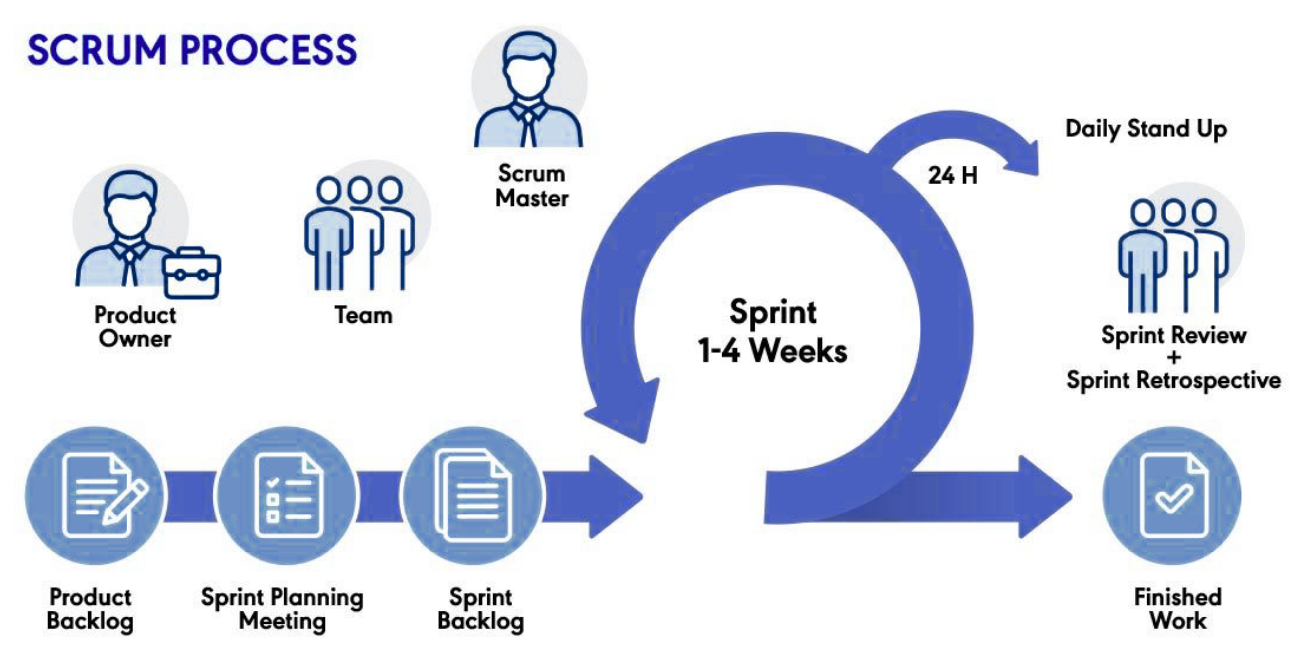
\includegraphics[width=0.8\linewidth]{figures/chapitre-01/scrum-process.png}
  \caption{Vue d’ensemble du processus Scrum.}
  \label{fig:doc-ch1-7}
\end{figure}

\subsubsection{Kanban}

Kanban est une méthode Agile orientée flux continu, basée sur la visualisation des tâches et la limitation du travail en cours. Les activités sont organisées dans un tableau composé de colonnes représentant les étapes du processus. Cette approche permet d’identifier rapidement les blocages, de fluidifier l’avancement et d’améliorer les délais de traitement \cite{kanban-method}.

La figure~\ref{fig:doc-ch1-8} présente une vue d’ensemble du processus Kanban.

\begin{figure}[H]
  \centering
  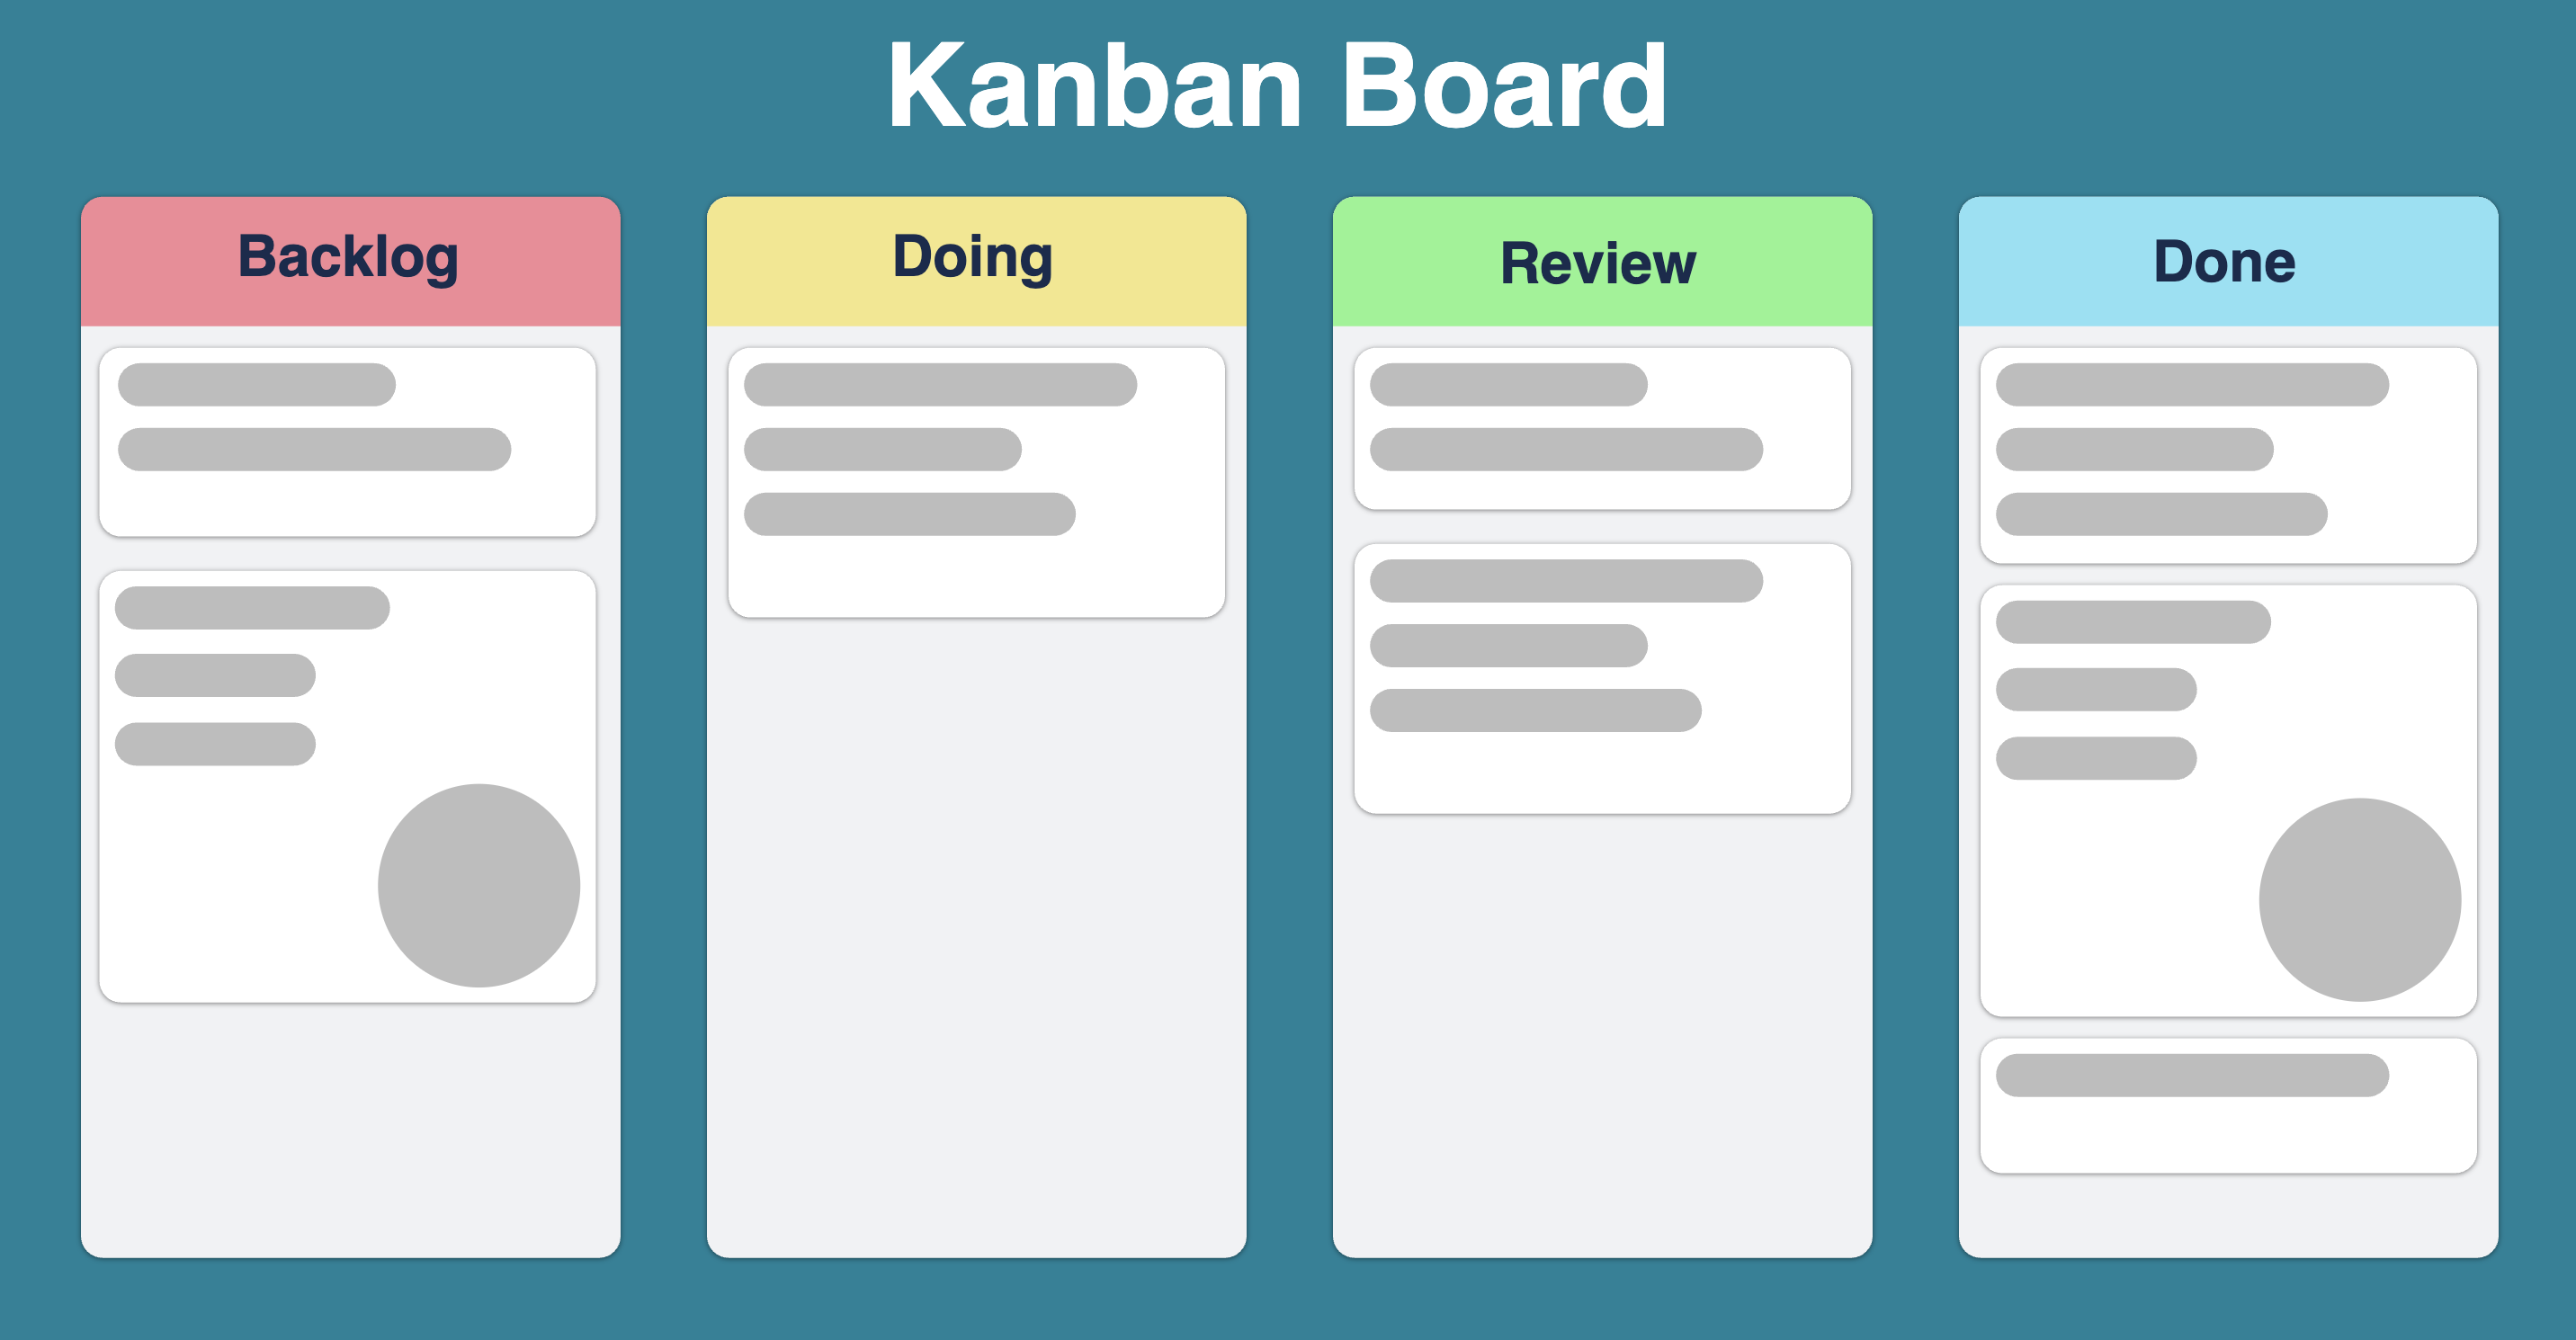
\includegraphics[width=0.7\linewidth]{figures/chapitre-01/kanban-process.png}
  \caption{Vue d’ensemble du processus Kanban.}
  \label{fig:doc-ch1-8}
\end{figure}
\subsubsection{Rational Unified Process (RUP)}

RUP est une méthodologie itérative et structurée basée sur quatre phases principales : inception, élaboration, construction et transition. Elle met l’accent sur la modélisation UML, la gestion des risques et une documentation détaillée \cite{sketchbubble-rup}.

Bien que RUP offre une bonne structuration du projet, sa complexité et sa lourdeur documentaire peuvent constituer un frein dans le cadre d’un projet académique à durée limitée.

La figure~\ref{fig:doc-ch1-9} illustre les phases principales de la méthodologie RUP.

\begin{figure}[H]
  \centering
  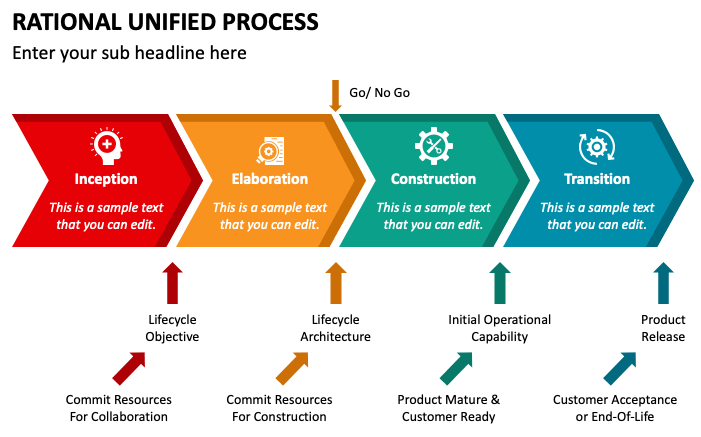
\includegraphics[width=0.92\linewidth]{figures/chapitre-01/rup-phases.png}
  \caption{Phases principales de la méthodologie RUP.}
  \label{fig:doc-ch1-9}
\end{figure}

\subsubsection{GIMSI}

GIMSI est une méthodologie de gestion de projets de systèmes d’information, souvent utilisée pour les projets de Business Intelligence et de tableaux de bord décisionnels. Elle vise à aligner les objectifs métier avec les indicateurs de performance \cite{headmind-bi-intro}.

Cette méthodologie est pertinente pour la partie reporting et indicateurs de performance, mais elle ne couvre pas de manière complète l’ensemble du cycle de développement logiciel.

La figure~\ref{fig:doc-ch1-10} présente les étapes principales de la méthodologie GIMSI.

\begin{figure}[H]
  \centering
  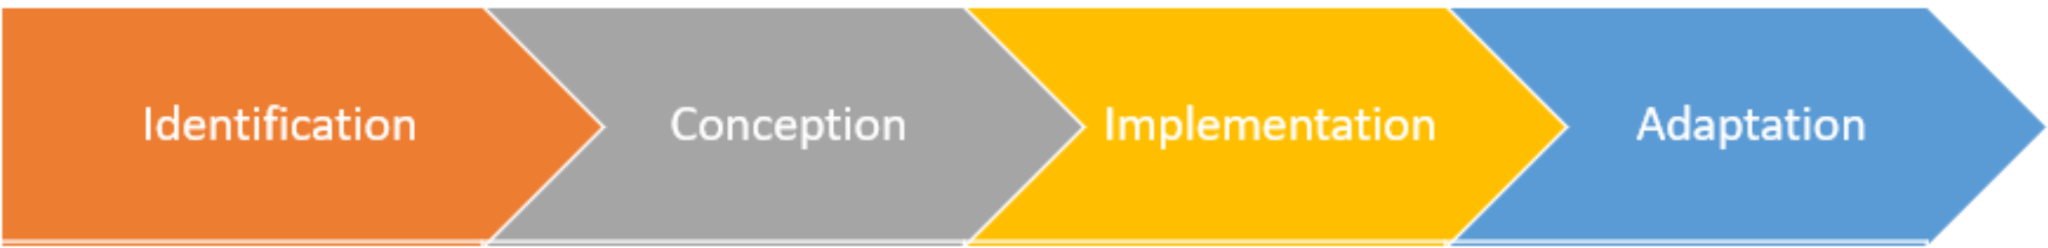
\includegraphics[width=0.92\linewidth]{figures/chapitre-01/gimsi-etapes-simplifiees.png}
  \caption{Étapes principales de la méthodologie GIMSI.}
  \label{fig:doc-ch1-10}
\end{figure}


\subsection{Comparaison des méthodologies}

Afin de sélectionner la méthodologie la plus adaptée au projet de Plateforme, plusieurs critères ont été définis en tenant compte des spécificités du projet, notamment la gestion multi-sites, l’évolution continue des besoins métier et l’intégration d’une forte composante Business Intelligence.

Les critères d’évaluation retenus sont les suivants :

\begin{itemize}[label=\textbullet, itemsep=0.15ex, parsep=0pt, topsep=0pt, partopsep=0pt]
  \item Orientation du méthodologie
  \item Structure et flexibilité
  \item Couverture du cycle SI
  \item Collaboration \& parties prenantes
  \item Scalabilité \& maintenabilité
  \item Adaptation au projet CSR
  \item Adaptation au BI \& décisionnel
\end{itemize}


\Needspace{22\baselineskip}%
Le tableau~\ref{tab:comparaison-methodes} présente une analyse comparative des méthodologies agiles étudiées.

\begin{table}[H]
  \centering
  \small
  \caption{Analyse comparative des méthodologies agiles étudiées}
  \label{tab:comparaison-methodes}
  \PFETableSetup
  \PFETableRowColors
  \PFETableArrayStretch
  \PFETableTabularXBegin
  \begin{tabularx}{\PFETableBlockWidth}{@{}%
    >{\raggedright\arraybackslash\hsize=0.95\hsize}X%
    >{\raggedright\arraybackslash\hsize=0.95\hsize}X%
    >{\raggedright\arraybackslash\hsize=0.95\hsize}X%
    >{\raggedright\arraybackslash\hsize=0.95\hsize}X%
    >{\raggedright\arraybackslash\hsize=0.95\hsize}X%
  @{}}
    \tableHeaderStyle \tableHeaderCell{Critères} &
    \tableHeaderCell{Scrum} &
    \tableHeaderCell{Kanban} &
    \tableHeaderCell{RUP} &
    \tableHeaderCell{GIMSI} \\

    Nombre d’étapes &
    5 étapes &
    Processus continu &
    4 étapes &
    4 étapes \\

    Étapes principales &
    Initialisation, Planification, Conception, Implémentation, Revue &
    Visualisation du flux, Limitation du travail en cours, Gestion continue du flux &
    Inception, Élaboration, Construction, Transition &
    Identification, Préparation, Implémentation, Évaluation \\

    Orientation &
    Développement logiciel agile &
    Gestion visuelle du flux de travail &
    Systèmes d’information &
    BI \& SI \\

    Structure &
    Flexible et itérative &
    Flexible et continue &
    Itérative et structurée &
    Hautement structurée \\

    Couverture du cycle SI &
    Élevée &
    Élevée &
    Très élevée &
    Élevée \\

    Collaboration des parties prenantes &
    Très élevée &
    Élevée &
    Élevée &
    Élevée \\

    Scalabilité \& maintenabilité &
    Élevée &
    Élevée &
    Élevée &
    Moyenne \\

    Adaptation au projet CSR &
    Très adaptée &
    Très adaptée &
    Adaptée &
    Adaptée \\

    Adéquation BI \& décisionnel &
    Adaptée &
    Moyenne &
    Moyenne &
    Très adaptée \\
  \end{tabularx}
  \PFETableTabularXEnd
\end{table}


\subsection{Méthodologie adoptée}

Sur la base de l’analyse comparative des méthodologies et en tenant compte de la nature hybride du projet, une approche combinée Scrum et GIMSI a été retenue.

Scrum sera utilisée pour le développement de la plateforme applicative CSR, permettant une livraison incrémentale des fonctionnalités, une prise en compte continue des retours utilisateurs et une forte collaboration entre les équipes techniques et métiers.

GIMSI sera adoptée pour la conception et la mise en œuvre de la couche Business Intelligence, notamment pour la définition des indicateurs clés (KPIs), la structuration des données, l’ETL\footnote{ETL : \emph{Extract, Transform, Load} (extraction, transformation et chargement des données). Il désigne le processus d’extraction des données depuis les systèmes sources, de leur transformation (nettoyage, règles métier, formats) et de leur chargement dans une zone ou un entrepôt destiné à l’analyse et au reporting.} et l’exploitation des tableaux de bord Power BI.

Cette combinaison méthodologique permet d’assurer la flexibilité et la réactivité face aux évolutions des besoins métier grâce à Scrum, tout en garantissant une démarche structurée et orientée décisionnel pour l’analyse et la valorisation des données CSR via GIMSI, ce qui favorise un alignement efficace de la plateforme opérationnelle avec les objectifs stratégiques et analytiques de COFICAB .

Ainsi, l’utilisation conjointe de Scrum et GIMSI constitue un choix pertinent et cohérent pour répondre aux exigences fonctionnelles, techniques et décisionnelles du projet.

\section{Conclusion}

Tout au long de ce chapitre, nous avons présenté le contexte de notre projet au sein  de la société COFICAB. Nous avons présenté la problématique, la mission et les objectifs du projet. Par ailleurs, nous avons mené une étude de l’existant et des solutions similaires avant d’esquisser la plateforme RSE proposée. Nous avons également comparé Scrum, RUP et GIMSI et retenu une approche hybride Scrum–GIMSI pour le développement et la partie décisionnelle. Dans le chapitre suivant, nous enchaînerons avec la fondation et l’initiation du projet.